\subsection{Cracking Minesweeper with SMT solver}
\label{minesweeper_SMT}

\renewcommand{\CURPATH}{equations/minesweeper/1_SMT}

For those who are not very good at playing Minesweeper (like me), it's possible to predict bombs' placement without touching debugger.

Here is a clicked somewhere and I see revealed empty cells and cells with known number of ``neighbours'':

\begin{figure}[H]
\centering
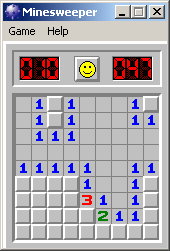
\includegraphics[scale=0.75]{\CURPATH/1.png}
\end{figure}

What we have here, actually? Hidden cells, empty cells (where bombs are not present), and empty cells with numbers, which shows how many bombs are placed nearby.

\subsubsection{The method}

Unlike many other examples, where our goal is to find a solution, here we use the fact that an instance is unsolvable (unsat).

Here is what we can do: we will try to place a bomb to all possible hidden cells and ask Z3 SMT solver,
if it can disprove the very fact that the bomb can be placed there.

Take a look at this fragment. "?" mark is for hidden cell, "." is for empty cell, number is a number of neighbours.

\begin{center}
\begin{tabular}{ | c | c | c | c | }
\hline
 & C1 & C2 & C3 \\
\hline
R1 & ? & ? & ? \\
\hline
R2 & ? & 3 & . \\
\hline
R3 & ? & 1 & . \\
\hline
\end{tabular}
\end{center}

So there are 5 hidden cells.
We will check each hidden cell by placing a bomb there.
Let's first pick top/left cell:

\begin{center}
\begin{tabular}{ | c | c | c | c | }
\hline
 & C1 & C2 & C3 \\
\hline
R1 & * & ? & ? \\
\hline
R2 & ? & 3 & . \\
\hline
R3 & ? & 1 & . \\
\hline
\end{tabular}
\end{center}

Then we will try to solve the following system of equations (\emph{RrCc} is cell of row $r$ and column $c$):

\begin{itemize}
\item R1C1=1                                         (because we placed bomb at R1C1)	
\item R2C1+R2C2+R2C3+R3C1+R3C2+R3C3=1                (because we have "1" at R3C2)	
\item R1C1+R1C2+R1C3+R2C1+R2C2+R2C3+R3C1+R3C2+R3C3=3 (because we have "3" at R2C2)	
\item R1C2+R1C3+R2C2+R2C3+R3C2+R3C3=0                (because we have "." at R2C3)	
\item R2C2+R2C3+R3C2+R3C3=0                          (because we have "." at R3C3)
\end{itemize}

As it turns out, this system of equations is satisfiable, so there could be a bomb at this cell.
But this information is not interesting to us, since we want to find cells we can freely click on.
And we will try another one.
And if the equation will be unsatisfiable, that would imply that a bomb cannot be there and we can click on it.

\subsubsection{The code}

\lstinputlisting[style=custompy]{\CURPATH/1.py}

The code is almost self-explanatory.
We need border for the same reason, why Conway's "Game of Life" implementations also has border (to make calculation
function simpler).
Whenever we know that the cell is free of bomb, we put zero there.
Whenever we know number of neighbours, we add a constraint, again, just like in "Game of Life": number of neighbours must be equal to the number we have seen in the Minesweeper.
Then we place bomb somewhere and check.

Based on map in the example, my script first tries to put a bomb at row=1 col=3 (first "?").
And this system of equations being generated:

\lstinputlisting{\CURPATH/r1_c3_expr.txt}

My script tries to solve the equation with no luck (unsat). That means, no bomb can be at that cell.

Now let's run it for all cells:

\begin{lstlisting}
row=1 col=3, unsat!
row=6 col=2, unsat!
row=6 col=3, unsat!
row=7 col=4, unsat!
row=7 col=9, unsat!
row=8 col=9, unsat!
\end{lstlisting}

These are cells where I can click safely, so I did:

\begin{figure}[H]
\centering
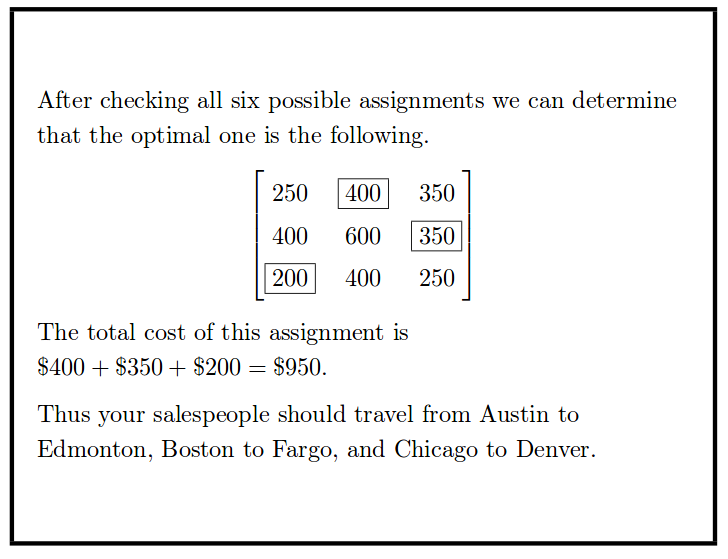
\includegraphics[scale=0.75]{\CURPATH/2.png}
\end{figure}

Now we have more information, so we update input:

\begin{lstlisting}
known=[
"01110001?",
"01?100011",
"011100000",
"000000000",
"111110011",
"?11?1001?",
"???331011",
"?????2110",
"???????10"]
\end{lstlisting}

I run it again:

\begin{lstlisting}
row=7 col=1, unsat!
row=7 col=2, unsat!
row=7 col=3, unsat!
row=8 col=3, unsat!
row=9 col=5, unsat!
row=9 col=6, unsat!
\end{lstlisting}

I click on these cells again:

\begin{figure}[H]
\centering
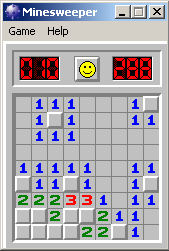
\includegraphics[scale=0.75]{\CURPATH/3.png}
\end{figure}

I update it again:

\begin{lstlisting}
known=[
"01110001?",
"01?100011",
"011100000",
"000000000",
"111110011",
"?11?1001?",
"222331011",
"??2??2110",
"????22?10"]
\end{lstlisting}

\begin{lstlisting}
row=8 col=2, unsat!
row=9 col=4, unsat!
\end{lstlisting}

\begin{figure}[H]
\centering
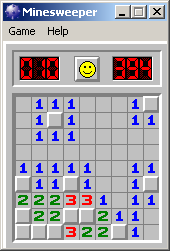
\includegraphics[scale=0.75]{\CURPATH/4.png}
\end{figure}

This is last update:

\begin{lstlisting}
known=[
"01110001?",
"01?100011",
"011100000",
"000000000",
"111110011",
"?11?1001?",
"222331011",
"?22??2110",
"???322?10"]
\end{lstlisting}

\dots last result:

\begin{lstlisting}
row=9 col=1, unsat!
row=9 col=2, unsat!
\end{lstlisting}

Voila!

\begin{figure}[H]
\centering
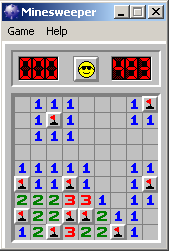
\includegraphics[scale=0.75]{\CURPATH/5.png}
\end{figure}

Some discussion on HN: \url{https://news.ycombinator.com/item?id=13797375}.

\subsubsection{More theory}

In Numb3rs TV series, Dr.Charlie Eppes tried to solve "Minesweeper game":
\url{https://en.wikipedia.org/wiki/Uncertainty_Principle_(Numbers)},
\url{http://pi.math.cornell.edu/~numb3rs/luthy/num104.html}.

What he is tried to do, is to find faster/better way to solve this game, by finding better methods to solve NP-problems in general.

Solving Minesweeper is NP-complete:
\url{http://simon.bailey.at/random/kaye.minesweeper.pdf},
\url{http://web.mat.bham.ac.uk/R.W.Kaye/minesw/ASE2003.pdf},
\url{http://math.oregonstate.edu/~math_reu/proceedings/REU_Proceedings/Proceedings2003/2003MK.pdf}.

Our way to solve it is also called "Minesweeper Consistency Problem"
\footnote{\url{https://www.claymath.org/sites/default/files/minesweeper.pdf}}.
We did it using system of integer equation.
And solving system of integer equation is NP-complete as well.

Find better way to solve Minesweeper, and you probably will be able to solve other NP-problems!

\subsubsection{Further reading}

Proofsweeper -- Play Minesweeper by formally proving your moves in Idris: \url{https://github.com/A1kmm/proofsweeper}.

